\chapter[Stručný manuál pro \LaTeXe]{Stručný manuál pro tvorbu AP v~publikačním systému \LaTeXe \label{ch:Manual_tex}}


V~této příloze je stručně uvedeno, jak vkládat do publikačního systému \LaTeXe\/ základní objekty (kapitoly, obrázky, tabulky, citace, křížové odkazy, rovnice atd.). Sledujte zdro\-jo\-vé kódy (soubory {\rm \texttt{*.tex}}). Tento text se nachází v~souboru \texttt{\cestaStyles Manual\_tex.tex}.



\section{Obrázky a~tabulky}


\subsection{Obrázky}

Obrázky do LaTeXu vkládáme ve formátu \verb"*.eps", které ukládáme do příslušných podadresářů \texttt{Figures}. Můžeme vkládat obrázky samostatně nebo vedle sebe jako \uv{podobrázky}.

\begin{figure}[H]
\begin{center}
    {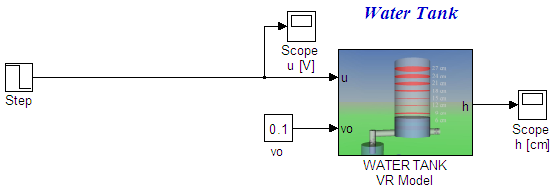
\includegraphics[height=4cm, angle=0]{\cestaStyles Figures/ModelWS}}
    \caption[Simulinkový model vodní nádrže -- převzato z~\protect\cite{Book:ROUBAL-HUSEK-kol_RTvP}]
        {Simulinkový model vodní nádrže -- převzato z~\protect\cite[Příloha\?: VR\_Toolbox\_Water.pdf]{Book:ROUBAL-HUSEK-kol_RTvP}}
    \label{fig:ModelWS}
\end{center}
\end{figure}

\begin{figure}[H]
\begin{center}
  \subfigure[napětí zubového čerpadla~$u$]
    {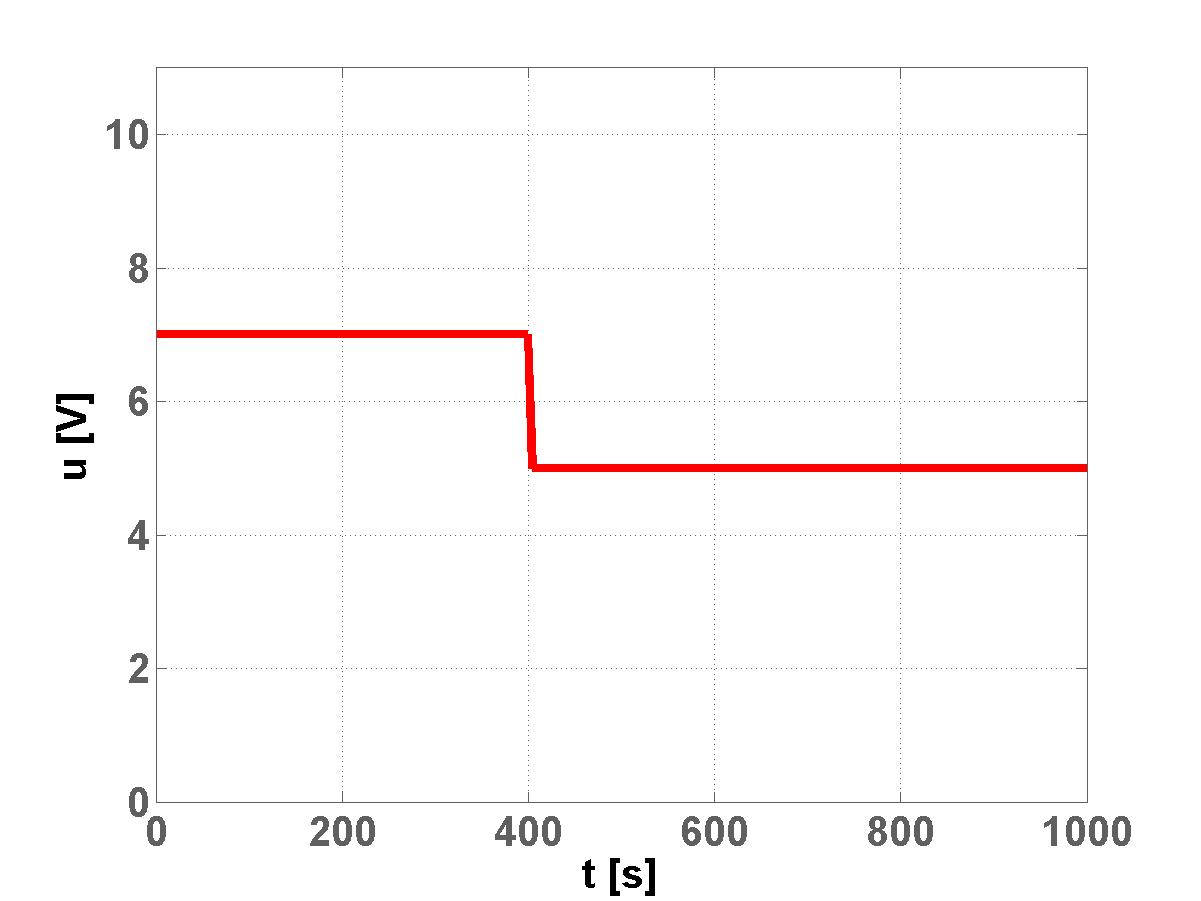
\includegraphics[width=7cm]{\cestaStyles Figures/Data_u}
    \label{fig:Data_u}}
  \hspace{1cm}
  \subfigure[výška hladiny v~nádrži~$h$]
    {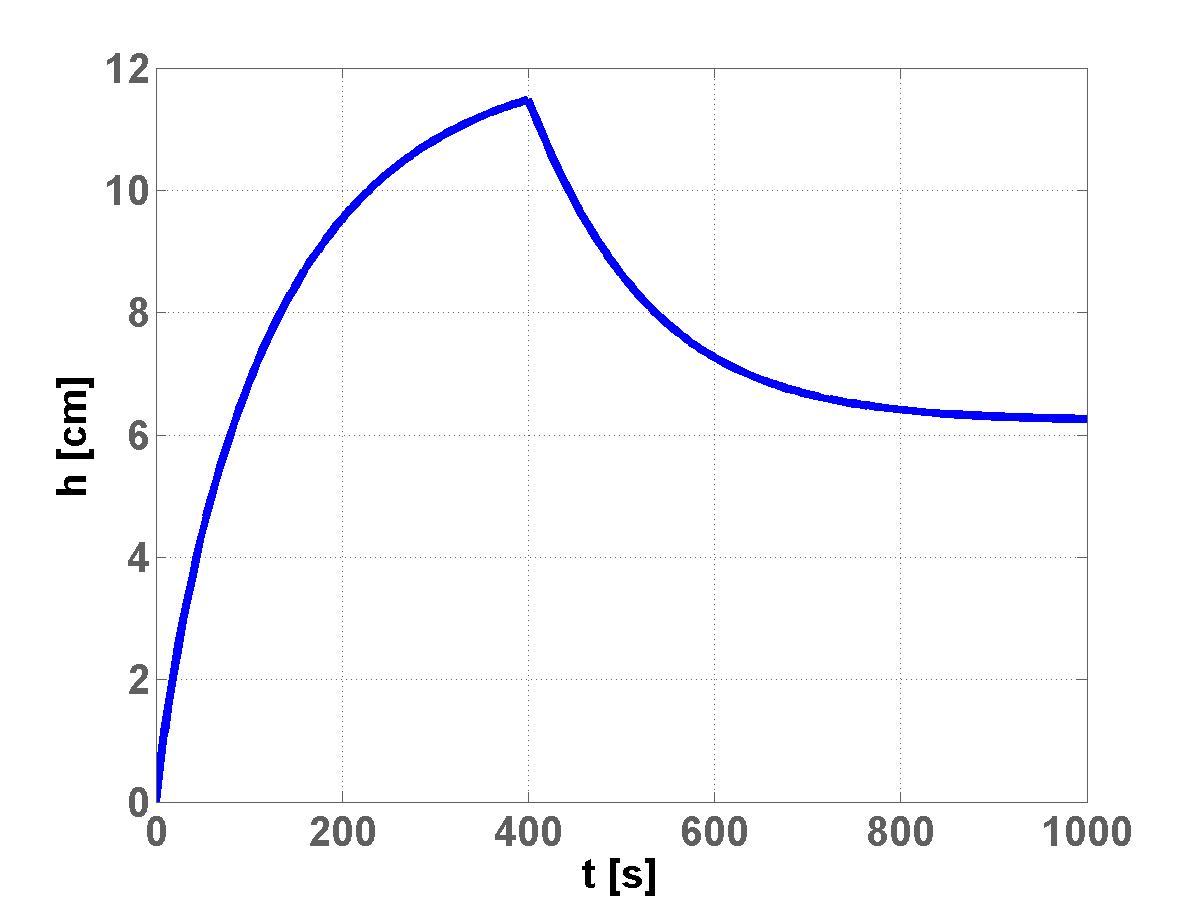
\includegraphics[width=7cm]{\cestaStyles Figures/Data_h}
    \label{fig:Data_h}}
  \caption[Časové odezvy virtuálního modelu vodní nádrže]
    {Časové odezvy virtuálního modelu vodní nádrže\protect\footnotemark}
  \label{fig:Data}
\end{center}
\end{figure}
\footnotetext{Obrázky převzaty
z~$\langle${\href{http://apps.copsu.cz/MoodleVOS/}{http://apps.copsu.cz/MoodleVOS/}}$\rangle$.}

Ta\-ké je možno vkládat obtékané obrázky s~popiskem. Ta\-ké je možno vkládat obtékané obrázky s~popiskem. Ta\-ké je možno vkládat obtékané obrázky s~popiskem. Ta\-ké je možno vkládat obtékané obrázky s~popiskem. Ta\-ké je možno vkládat obtékané obrázky s~popiskem. Ta\-ké je možno vkládat obtékané obrázky s~popiskem. Ta\-ké je možno vkládat obtékané obrázky s~popiskem. Ta\-ké je možno vkládat obtékané obrázky s~popiskem. Ta\-ké je možno vkládat obtékané obrázky s~popiskem. Ta\-ké je možno vkládat obtékané obrázky s~popiskem. Ta\-ké je možno vkládat obtékané obrázky
s~popiskem.

\begin{wrapfigure}[13]{i}{6.5cm}
\begin{center}
  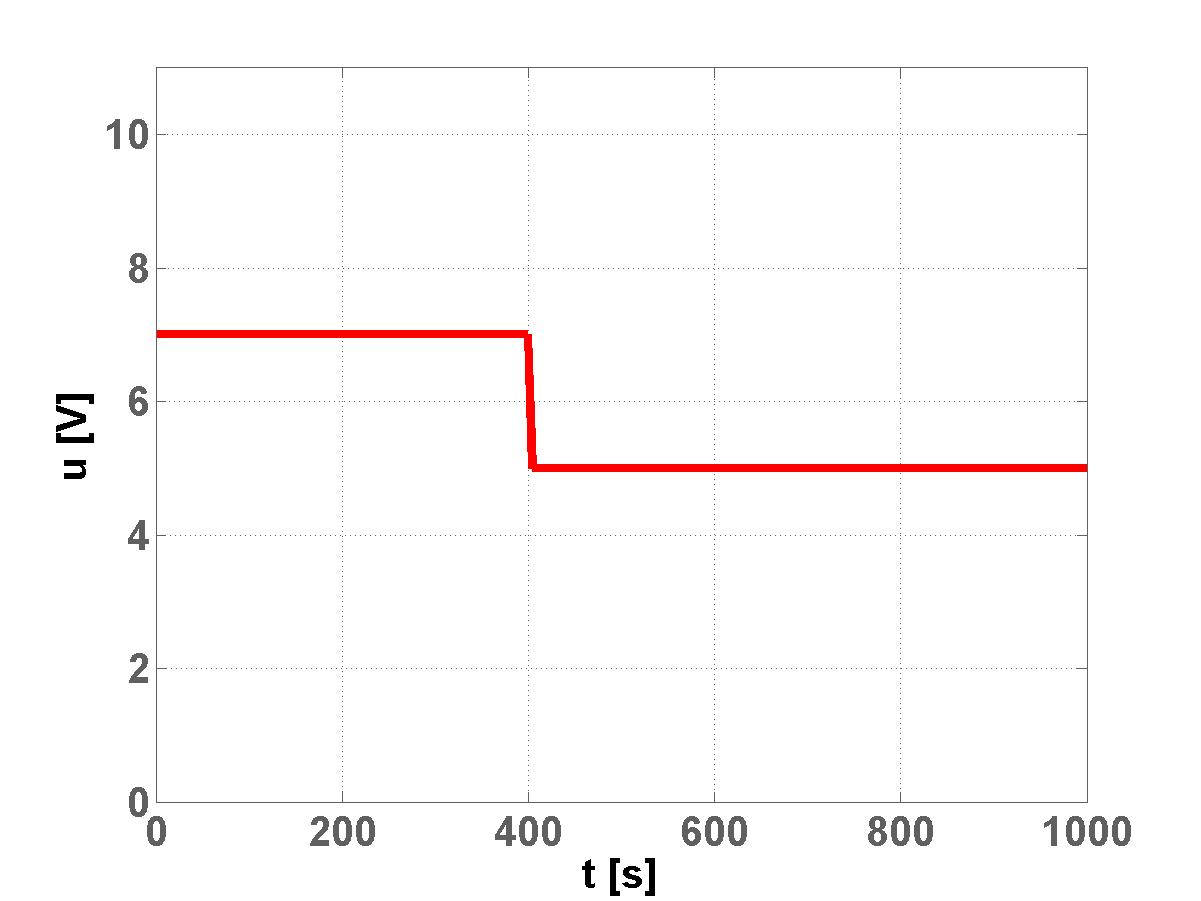
\includegraphics[width=6cm]{\cestaStyles Figures/Data_u}
  \caption{Obtékáný obrázek}
  \label{fig:Data_u2}
\end{center}
\end{wrapfigure}
V~tom pří\-pa\-dě dej\-te po\-zor na dě\-le\-ní slov. V~tom pří\-pa\-dě dej\-te po\-zor na dě\-le\-ní slov. V~tom pří\-pa\-dě dej\-te po\-zor na dě\-le\-ní slov. V~tom pří\-pa\-dě dej\-te po\-zor na dě\-le\-ní slov. V~tom pří\-pa\-dě dej\-te po\-zor na dě\-le\-ní slov. V~tom pří\-pa\-dě dej\-te po\-zor na dě\-le\-ní slov. V~tom pří\-pa\-dě dej\-te po\-zor na dě\-le\-ní slov. V~tom pří\-pa\-dě dej\-te po\-zor na dě\-le\-ní slov. V~tom pří\-pa\-dě dej\-te po\-zor na dě\-le\-ní slov. V~tom pří\-pa\-dě dej\-te po\-zor na dě\-le\-ní slov. V~tom pří\-pa\-dě dej\-te po\-zor na dě\-le\-ní slov. V~tom pří\-pa\-dě dej\-te po\-zor na dě\-le\-ní slov. V~tom pří\-pa\-dě dej\-te po\-zor na dě\-le\-ní slov. V~tom pří\-pa\-dě dej\-te po\-zor na dě\-le\-ní slov. V~tom pří\-pa\-dě dej\-te po\-zor na dě\-le\-ní slov. V~tom pří\-pa\-dě dej\-te po\-zor na dě\-le\-ní slov. V~tom pří\-pa\-dě dej\-te po\-zor na dě\-le\-ní slov. V~tom pří\-pa\-dě dej\-te po\-zor na dě\-le\-ní slov. V~tom pří\-pa\-dě dej\-te po\-zor na dě\-le\-ní slov. V~tom pří\-pa\-dě dej\-te po\-zor na dě\-le\-ní slov. V~tom pří\-pa\-dě dej\-te po\-zor na dě\-le\-ní slov. V~tom pří\-pa\-dě dej\-te po\-zor na dě\-le\-ní slov. V~tom pří\-pa\-dě dej\-te po\-zor na dě\-le\-ní slov. V~tom pří\-pa\-dě dej\-te po\-zor na dě\-le\-ní slov. V~tom pří\-pa\-dě dej\-te po\-zor na dě\-le\-ní slov. V~tom pří\-pa\-dě dej\-te po\-zor na dě\-le\-ní slov. V~tom pří\-pa\-dě dej\-te po\-zor na dě\-le\-ní slov. V~tom pří\-pa\-dě dej\-te po\-zor na dě\-le\-ní slov. V~tom pří\-pa\-dě dej\-te po\-zor na dě\-le\-ní slov. V~tom pří\-pa\-dě dej\-te po\-zor na dě\-le\-ní slov. V~tom pří\-pa\-dě dej\-te po\-zor na dě\-le\-ní slov. V~tom pří\-pa\-dě dej\-te po\-zor na dě\-le\-ní slov.


\subsection{Tabulky}

\begin{table}[H]
  \centering
  \caption{Obyčejná tabulka}\label{tab:values}
  \begin{tabular}{|l|c|r|}
    % after \\: \hline or \cline{col1-col2} \cline{col3-col4} ...
    \hline
    \textbf{Fyzikální veličina} & \textbf{Označení} & \textbf{Jednotka} \\ \hline
    {napětí na čerpadle}        & {$u$}             & {V}               \\ \hline
    {plocha podstavy nádrže}    & {$S$}             & {m$^2$}           \\ \hline
    {hustota}                   & {$\rho$}          & {kg\,m$^{-3}$}    \\ \hline
  \end{tabular}
\end{table}

\begin{table}[H]
  \centering
  \caption{Tabulka s dlouhými texty}\label{tab:text}
  \begin{tabular}{|p{9cm}|p{6cm}|}
    % after \\: \hline or \cline{col1-col2} \cline{col3-col4} ...
    \hline
    {co když je text v~1.~buňce strašně dlouhý, co když je text v~1.~buňce strašně dlouhý, co když je text v~1.~buňce strašně dlouhý}
        & {co když je text ve 2.~buňce strašně dlouhý}
        \\ \hline
    \parbox{5cm}{co když je text v~1.~buňce strašně dlouhý, co když je text v~1.~buňce strašně dlouhý, co když je text v~1.~buňce strašně dlouhý, co když je text v~1.~buňce strašně dlouhý, co když je text v~1.~buňce strašně dlouhý, co když je text v~1.~buňce strašně dlouhý, co když je text v~1.~buňce strašně dlouhý}
        & {co když je text ve 2.~buňce strašně dlouhý}
        \\ \hline
  \end{tabular}
\end{table}

\begin{table}[H]
  \catcode`\-=12
  \centering
  \caption{Tabulka se sloučenými buňkami}\label{tab:cells}
  \begin{tabular}{|l|c|c|}
    \hline
    {}                          & \multicolumn{2}{|c|}
                                    {\textbf{Fyzikální veličina}}       \\ \cline{2-3}
    \textbf{Popis}              & \textbf{označení} & \textbf{jednotka} \\ \hline
    {napětí na čerpadle}        & {$u$}             & {V}               \\ \hline
    {plocha podstavy nádrže}    & {$S$}             & {m$^2$}           \\ \hline
    {hustota}                   & {$\rho$}          & {kg\,m$^{-3}$}    \\ \hline
  \end{tabular}
\end{table}



\section{Křížové odkazy a~poznámky pod čarou}

Pro tvorbu křížových odkazů je třeba použít příkazy \verb"\label{}" a \verb"\ref{}", respektive pro citace příkaz
\verb"\cite{}", viz ná\-sle\-du\-jí\-cí příklady.

\begin{itemize}
    \item v~kapitole~\ref{ch:Uvod}
    \item Poznámky pod čarou se tvoří takto\footnote{Poznámka pod čarou je asi věta.}. Před číslem (horním indexem) není mezera.
    \item na~\figref{fig:ModelWS} nebo na~\figref{fig:Data_h}\footnote{Jak se píší poznámky pod čarou k~popisu obrázku se podívejte na~\figref{fig:Data}.}
    \item viz~\tabref{tab:values},
    \item podle rovnice~\eqref{eq:rovnice1},
    \item na literaturu, konkrétně
    \begin{itemize}
        \item na knihu~\cite{Book:ROUBAL-HUSEK-kol_RTvP},
        \item na část knihy~\cite[strana~10]{Book:ROUBAL-HUSEK-kol_RTvP}\footnote{Jak se cituje literatura v~popisu obrázku se podívejte
                na~\figref{fig:ModelWS}.},
        \item na článek v~časopise~\cite{Article:ROUBAL-HUSEK-STECHA_LSFOP},
        \item na web~\cite{WWW_Lab26},
        \item na diplomku~\cite{MastersThesis:ROUBAL_BP} nebo absolventské práce~\cite{AbsolventThesis:SIKYR_AP,AbsolventThesis:BOSTICKA_AP,AbsolventThesis:RABINAK_AP,AbsolventThesis:PAVLAT_AP},
    \end{itemize}
        seznam literatury je automaticky vygenerován za poslední kapitolou (před první přílohou),
    \item na definici~\ref{de:definice1}, větu~\ref{pr:veta1}, příklad~\ref{ex:priklad1}.
\end{itemize}



\section{Rovnice}

Rovnice je možné psát ručně přímo zde, nebo pomocí programu TeXaide, který je podobný editoru rovnic v~MS Word. Najdete ho zdarma na internetu.

Rovnice v~textu píšeme takto $y = 0\.5 x + 10$ (pozor na fonty, musí být stejné jako u~\uv{normálních} níže uvedených rovnic). V~\LaTeX\!\,u stačí dát výraz mezi dolary (\$ \$). Pro desetinnou čárku používáme \verb"\." -- jinak by se za čárkou objevila nežádoucí mezera podobně jako ve větách.


\subsection{Veličina, hodnota a fyzikální jednotka}

Fyzikální jednotky se nepíší kurzívou. Hodnota a~její jednotka se nesmí rozdělit na konci řádku. Správný zápis, se správně nastavenými mezerami mezi hodnotou a~jednotkou, je $u = 568\.3\,$mV. Což se TeXovsky zapíše takto
    \[
    \verb"$u = 568\.3\,$mV".
    \]


\subsection{Nečíslované rovnice}

    \[
    y = 0\.5 x + 10
    \]


\subsection{Číslované rovnice}

\begin{equation}\label{eq:rovnice1}
    y = 0\.5 x + 5
\end{equation}


\subsection{Maticové rovnice}

Maticové rovnice píšeme takto
\begin{equation}\label{eq:rovnice2}
    \mat{A} = \mat{B} + \mat{C},
\end{equation}
nebo takto
\begin{equation}\label{eq:rovnice3}
    \left[ \begin{array}{l}
        \dot x_1 (t) \\
        \dot x_2 (t) \\
    \end{array} \right] =
    \left[ {\begin{array}{*{20}c}
        1 & 1  \\
        0 & 2  \\
    \end{array}} \right]
    \left[ \begin{array}{l}
        x_1 (t) \\
        x_2 (t) \\
    \end{array} \right]\!.
\end{equation}
Nezapomeňte, že rovnice je součástí věty a~píšeme za ní čárky nebo tečky, jako v~nor\-mál\-ní slovní větě.



\section{Zdrojové kódy například z~Matlabu}

Takto je možné vkládat zdrojové kódy z~programovacích jazyků.
\begin{matlab}{.9\linewidth}{dgreen}
    %% Komentář ke kódu
    clc;
    clear;
    close all;

    omega = 1;
    jmn = [1 2*zeta*omega omega^2];

    figure(1);
        for zeta = 1E-5 : 0.2 : 1+1E-12
            G = tf(omega^2,subs([1 2*zeta*omega omega^2]));
            bode(G);
            hold on;
        end
        grid on;
    legend('\zeta = 0','\zeta = 0,2','\zeta = 0,4','\zeta = 0,6','\zeta = 0,8','\zeta = 1');
    text(1.1,230,'\infty','FontSize',16,'FontWeight','bold');
\end{matlab}
Pokud chcete změnit velikost písma, předefinujte jej v~příslušném souboru \texttt{\cestaStyles *.sty} na řádce~267.

Pokud chcete zachovat barvy kódu, pak použijte následující způsob. Podívejte se na zdrojový kód do souboru \texttt{\cestaStyles Manual\_tex.tex}. Pro změnu programovacího jazyka je nutno předefinovat v~příslušném souboru \texttt{\cestaStyles *.sty} na řádek~278.

\begin{lstlisting}
    %% Komentář ke kódu
    clc;
    clear;
    close all;

    omega = 1;
    jmn = [1 2*zeta*omega omega^2];

    figure(1);
        for zeta = 1E-5 : 0.2 : 1+1E-12
            G = tf(omega^2,subs([1 2*zeta*omega omega^2]));
            bode(G);
            hold on;
        end
        grid on;
    legend('\zeta = 0','\zeta = 0,2','\zeta = 0,4','\zeta = 0,6','\zeta = 0,8','\zeta = 1');
    text(1.1,230,'\infty','FontSize',16,'FontWeight','bold');
\end{lstlisting}



\section{Slova do rejstříku}


\index{Slovo do rejstříku 1}

\index{Slovo do rejstříku 2}

\index{charakteristika}

\index{charakteristika!přechodová}

\index{charakteristika!frekvenční}


Slova do rejstříku vkládáme pomocí klíčového slova \texttt{$\backslash$index\{\}}, do kterého napíšeme na patřičném místě v textu dané klíčové slovo, viz zdrojový text v~\texttt{\cestaStyles Manual\_tex.tex}.



\section{Definice, věty, příklady ...}

\begin{definition}[Název definice]\label{de:definice1}
Takto se píší definice.
\end{definition}

\begin{proposition}[Název věty]\label{pr:veta1}
Takto se píší věty.
\end{proposition}

\begin{example}[Název příkladu]\label{ex:priklad1}
Takto se píší příklady.
\end{example}
\begin{solution}
Takto je možné psát řešení příkladu.
\end{solution}

\begin{note}
Takto se píší poznámky.
\end{note}

\begin{proof}
Takto se píší důkazy.
\end{proof}



\textcolor{blue}{\em Tento text se nachází v~souboru \texttt{\cestaStyles Manual\_Tex.tex}. Pro odstranění této přílohy zakomentujte v~souboru \texttt{Diplomka.tex} řádek~170, respektive v~souboru \texttt{MP.tex} řádek~180, respektive v~souboru \texttt{SOC.tex} řádek~180\?: \texttt{$\backslash$input$\{$\cestaStyles Manual\_tex.tex$\}$}.\/}
